\section{Attack Taxonomy}\label{attack}


Other than membership inference inference attacks in Graph NNs as described in [], we propose four novel attack surfaces for Graph models based on the leakage from graph embeddings.

\begin{figure}[!htb]
\centering
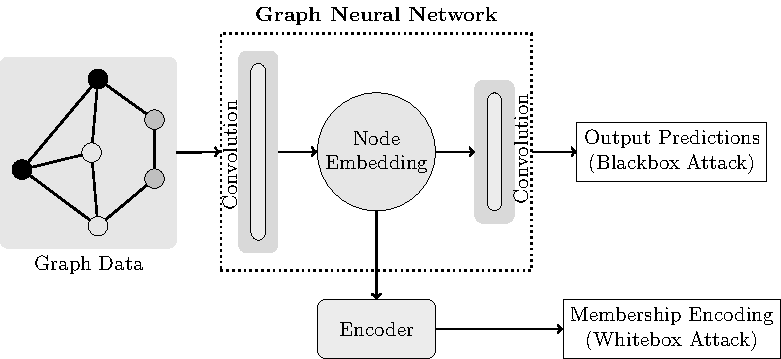
\includegraphics[width=0.85\linewidth]{./figures/Attacks/MIA.pdf}
\caption{Example of a parametric}
\end{figure}



\begin{figure}
    \centering
    \begin{minipage}[b]{1\linewidth}
    \centering

    \subfigure[Output Distribution for all records]{
   	\label{fig:mem_soft_label}
    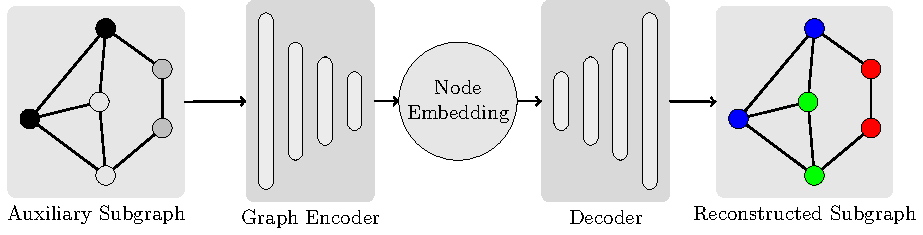
\includegraphics[width=\linewidth]{./figures/Attacks/reconstruction.pdf}
    }

    \subfigure[Output Distribution for all records]{
    \label{fig:mem_soft_label}
    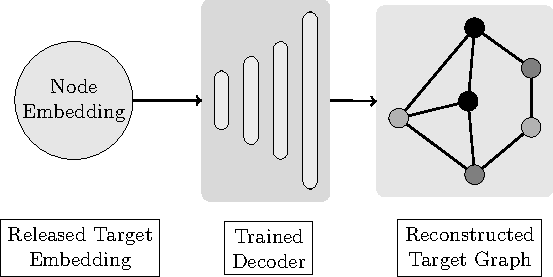
\includegraphics[width=0.6\linewidth]{./figures/Attacks/reconstruction2.pdf}
    }
    \end{minipage}
    \caption{Distribution of the confidence score vectors of the target classifier on the training data and test data of class 29 in the Purchase100 dataset. Each color represents one data record.}
    \label{fig:soft_label}
\end{figure}



Threat Model: blackbox..

Adversary prior Knowledge

\subsection{Graph Reconstruction Attack}

Adversary Goal

Attack Methodology

\subsection{Stealing Model Functionality}


\subsection{Link Inference Attack}

Link Inference attacks is a binary classification problem where the adversary aims to infer whether there exists a links between two nodes in the graph.
This translates to identifying whether two people know each other in case of online social networks and identifying the friendship circle which can violate the privacy of the individual.
Link Inference attacks naturally follow from the reconstruction attack where given the reconstructed graph, the adversary can check for an edge between two users using the adjacency matrix.
Write link inference as checking the adjacency matrix...


\subsection{Attribute Inference Attack}

Given an embedding of the graph node $\Psi$

Adversary Goal

Attack Methodology



\subsection{Embedding MIA}

The adversary in a whitebox setting has access to the model output predictions $f(x; W)$ for an input $x$ as well as the model parameters $W$.
This allows the adversary to compute the intermediate computations after each layer.
This is a strong adversary assumption but practical in cases such as federated learning where the intermediate computations and parameters can be observed~\cite{8835245,DBLP:conf/sp/MelisSCS19}.

%\noindent\textbf{Attack Motivation.}
As explained Section~\ref{graphnn}, GNNs compute the low dimensional feature embedding for the input graph data.
The parameters of the embedding function are updated in each iteration of training and tuned specifically for high performance on the train data resulting in a distinguishable footprint between feature embedding of train and test data points.
Figure~\ref{embedding} illustrates this rationale by plotting feature embedding of train and test records for the three datasets after a dimension reduction using 2D-TSNE algorithm~\cite{vanDerMaaten2008}.



%\noindent\textbf{Attack Methodology.}
The attack is unsupervised since we assume the adversary has no prior knowledge to map the intermediate feature embeddings to a membership value. % (available as auxiliary knowledge in shadow model).
The adversary trains an encoder-decoder network in unsupervised fashion to map the intermediate embedding to a single membership value.
For an input $x$, encoder $f_{enc}()$ generates a scalar membership value which is passed to decoder $f_{dec}(f_{enc}(x))$ to obtain $x$ by minmizing reconstruction loss: $||x - f_{dec}(f_{enc}(x))||_2^2$.
Given the membership values for different training and testing data points, K-Means clustering is used to cluster the nodes into two classes (members and non-members).
For any new input, the adversary can then use this clustering to map it as members or non-members of the training data.
This novel whitebox attack exploits the difference in embedding representation between members and non-members of training data which is not possible for Deep Neural Networks trained on euclidean data where the intermediate activations are abstract (generalize well) and cannot be used to distinguish members and non-members~\cite{8835245}.
